\documentclass[12pt]{exam}
\newcommand{\semanticversion}{v1.3.0}               % release version
\newcommand{\studentone}{Gage C. Linville}			% enter your name
%\newcommand{\studentemail}{}			            % enter your student email
%\newcommand{\studentwebsite}{Visit soils.land for more resources}                     % enter your website
\title{Soil Horizons Cheat Sheet}					% change to the title of the project
\author{\studentone}				                % you don't have to change this
% Creation date
\newcommand{\creationdate}{April 5th, 2023}
% Revision date
\newcommand{\revisiondate}{May 13th, 2023}

%-------------------------------------------------------------------------------------
%  PACKAGES
%-------------------------------------------------------------------------------------
\usepackage{graphicx}
\usepackage{siunitx}
\usepackage{amsmath}
\usepackage{array}
\usepackage{enumitem}

%-------------------------------------------------------------------------------------
%  GRAPHICS PATH
%-------------------------------------------------------------------------------------
\graphicspath{{figures/}}								% put your figures in a folder called figures

%---------------------------------------------------------------------------
% FUNCTIONS FOR IMPORTING FIGURES
%---------------------------------------------------------------------------
\newcommand{\placefigure}[1]{\centerline{\includegraphics[width=2 in]{#1}}}
\newcommand{\placefigureandscale}[2]{\centerline{\includegraphics[width=#2 in]{#1}}}

%-------------------------------------------------------------------------------------
% TITLE PAGE MACRO
%-------------------------------------------------------------------------------------
\makeatletter
\def\maketitle{%
  \null
  \thispagestyle{empty}
  \begin{center}\leavevmode
       \normalfont
       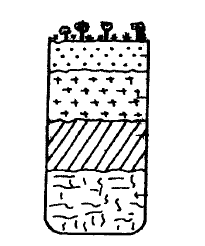
\includegraphics[width=0.20\columnwidth]{figures/Image_Edit.png}
%       \vskip 0.5cm
%       \textsc{\Large soils.land}\\[0.2 cm]
%       \vskip 0.3cm
	\rule{\linewidth}{0.2 mm} \\[0.4 cm]
	{ \huge \bfseries \@title}\\
	\rule{\linewidth}{0.2 mm} \\[0.4 cm]

	\begin{minipage}{0.5\textwidth}
		 \begin{center}\large
			Compiled by: \studentone\\
            Created: \creationdate\\
            Revised: \revisiondate\\
            \semanticversion\\
%			\studentemail\\
           \studentwebsite
			\end{center}
			\end{minipage}
   \end{center}
   \vfill
   \null
   \cleardoublepage
  }
\makeatother

%-------------------------------------------------------------------------------------
%	START OF DOCUMENT
%-------------------------------------------------------------------------------------

\begin{document}
%\large
\maketitle
%\frontmatter
\let\cleardoublepage\clearpage
%\mainmatter
\sloppy

%-------------------------------------------------------------------------------------
% CONTENTS
%-------------------------------------------------------------------------------------

\begin{center}
   \section*{Master Horizons}
\end{center}
 \hrulefill

\begin{description}[labelsep=2.45em, align=right]
\item[O]
Predominantly organic material, leaves, moss, and other plant materials may be identifiable or may be extensively altered.
\vspace{0.1in}
\item[A]
Predominantly mineral, mixed with lesser amounts of accumulated organic matter. Typically a surface horizon but often below an \textbf{O} horizon.
\vspace{0.1in}
\item[B]
Subsurface horizon with illuvial (washed in) accumulation of one or more clay, Fe, Al, Si, humus, carbonates, gypsum, or a horizon with other specific subsoil features.
\vspace{0.1in}
\item[C]
Parent material, unconsolidated earthy material with little or no evidence of horizon development or pedogenic alteration.
\vspace{0.1in}
\item[E]
Mineral horizon, usually light in color, from which some combination of fine clays, Fe, Al, and organic matter has been eluviated (washed out).
\vspace{0.1in}
\item[L]
Limnic layer including organic and inorganic materials deposited through the actions of aquatic organisms.
\vspace{0.1in}
\item[M]
Root-limiting layer of human-manufactured material such as asphalt, concrete, or plastic.
\vspace{0.1in}
\item[R]
Continuous bedrock, too hard for hand-digging with a spade.
\vspace{0.1in}
\item[V]
Mineral horizons formed at the soil surface or below a layer of rock fragments. They are characterized by the predominance of vesicular pores and have platy, prismatic, or columnar structure.
\vspace{0.1in}
\item[W]
Rarely used. A layer of liquid or frozen water within or beneath, but not above, the soil.
\vspace{0.1in}
\item[AE]
Transition horizon, dominated by properties of an \textbf{A} horizon with subordinate properties of an \textbf{E} horizon. Similarly, the first letter designates the dominant properties in other transition horizons: \textbf{AB,} \textbf{BA,} \textbf{BE,} \textbf{EA,} \textbf{EB,} \textbf{BC,} and \textbf{CB.}
\vspace{0.1in}
\item[A/E]
Combination horizon, dominated by properties of an \textbf{A} horizon with discrete intermingled bodies of \textbf{E} horizon. Similarly, the first letter designates the dominant horizon in other combination horizons: \textbf{A/B,} \textbf{A/C,} \textbf{B/A,} \textbf{B/E,} \textbf{B/C,} \textbf{E/A,} \textbf{E/B,} \textbf{C/A,} and \textbf{C/B.}
\end{description}

\newpage
\begin{center}
    \section*{Suffixes}
\end{center}
    \hrulefill

\begin{description}[labelsep=1.80em, align=right]
\item[a]
Highly decomposed organic matter. Example: \textbf{Oa.}
\vspace{0.1in}
\item[b]
Buried horizon that developed before burial. Example: \textbf{Ab.}
\vspace{0.1in}
\item[c]
Concretions or nodules. Example: \textbf{Bc.}
\vspace{0.1in}
\item[co]
Coprogenous earth (sedimentary peat). Example: \textbf{Lco.}
\vspace{0.1in}
\item[d]
Dense horizon physically restricting roots. Example: \textbf{Bd.}
\vspace{0.1in}
\item[di]
Diatomaceous earth. Example: \textbf{Ldi.}
\vspace{0.1in}
\item[e]
Organic material of intermediate decomposition. Example: \textbf{Oe.}
\vspace{0.1in}
\item[f]
Frozen soil or water. Example: \textbf{Wf.}
\vspace{0.1in}
\item[ff]
Dry permafrost, permanently below 0°C, but little water present. Example: \textbf{Aff.}
\vspace{0.1in}
\item[g]
Strong gleying, iron is reduced, usually having a chroma below 2. Example: \textbf{Cg.}
\vspace{0.1in}
\item[h]
Illuvial accumulation of organic matter. Example: \textbf{Bh.}
\vspace{0.1in}
\item[i]
Slightly decomposed organic matter. Example: \textbf{Oi.}
\vspace{0.1in}
\item[j]
Accumulation of jarosite, a yellow sulfate mineral. Example: \textbf{Bj.}
\vspace{0.1in}
\item[jj]
Evidence of cryoturbation (soil horizon disruption from freezing). Example: \textbf{Ajj.}
\vspace{0.1in}
\item[k]
Accumulation of carbonates. Example: \textbf{Bk.}
\vspace{0.1in}
\item[kk]
Engulfment of horizon by secondary carbonates. Example: \textbf{Bkk.}
\vspace{0.1in}
\item[m]
Pedogenic cementation. Example: \textbf{Bm.}
\vspace{0.1in}
\item[ma]
Marl. Example: \textbf{Lma.}
\vspace{0.1in}
\item[n]
Accumulation of sodium. Example: \textbf{Bn.}
\vspace{0.1in}
\item[o]
Residual accumulation of sesquioxides. Example: \textbf{Bo.}
\vspace{0.1in}
\item[p]
Tillage or other disturbance of the surface soil. Example: \textbf{Ap.}
\vspace{0.1in}
\item[q]
Accumulation of silica. Example: \textbf{Bq.}
\vspace{0.1in}
\item[r]
Weathered or soft bedrock. Example: \textbf{Cr.}
\vspace{0.1in}
\item[s]
Illuvial accumulation of metals complexed with organic matter. Examples: \textbf{Bs.}
\vspace{0.1in}
\item[se]
Presence of sulfides. Example: \textbf{Bse.}
\vspace{0.1in}
\item[ss]
Slickensides. Example: \textbf{Bss.}
\vspace{0.1in}
\item[t]
Accumulation of silicate clay. Example: \textbf{Bt.}
\vspace{0.1in}
\item[u]
Presence of human-manufactured materials (artifacts). Example: \textbf{Au.}
\vspace{0.1in}
\item[v]
Plinthite. Example: \textbf{Bv.}
\vspace{0.1in}
\item[w]
Development of color or structure, without accumulation of colloids. Example: \textbf{Bw.}
\vspace{0.1in}
\item[x]
Fragipan, dense, firm, and brittle. Example: \textbf{Bx.}
\vspace{0.1in}
\item[y]
Accumulation of gypsum. Example: \textbf{By.}
\vspace{0.1in}
\item[yy]
Dominance of horizon by gypsum. Example: \textbf{Byy.}
\vspace{0.1in}
\item[z]
Accumulation of salts more soluble than gypsum. Example: \textbf{Bz.}
\vspace{0.2in}

\textbf{References:}\\
1. Gardiner, Duane T., and Raymond W. Miller. Soils in Our Environment. Pearson Prentice Hall, 2008.\\
2. Soil Survey Staff. 2022. Keys to Soil Taxonomy, 13th ed. USDA-Natural Resources Conservation Service.
% https://www.nrcs.usda.gov/resources/guides-and-instructions/keys-to-soil-taxonomy#keys
\end{description}
\end{document}
